\documentclass[a4paper,12pt]{article}
\usepackage[margin=1in]{geometry}
\usepackage{graphicx}
\usepackage{longtable}
\usepackage{caption}
\usepackage{listings}
\usepackage{xcolor}
\usepackage{float}
\usepackage{hyperref}

\definecolor{dkgreen}{rgb}{0,0.6,0}
\definecolor{gray}{rgb}{0.5,0.5,0.5}
\definecolor{mauve}{rgb}{0.58,0,0.82}

\lstset{
  frame=tb,
  language=Java,
  aboveskip=3mm,
  belowskip=3mm,
  showstringspaces=false,
  columns=flexible,
  basicstyle={\small\ttfamily},
  numbers=none,
  numberstyle=\tiny\color{gray},
  keywordstyle=\color{blue},
  commentstyle=\color{dkgreen},
  stringstyle=\color{mauve},
  breaklines=true,
  breakatwhitespace=true,
  tabsize=3,
  backgroundcolor=\color{gray!10}
}

\title{Lab 2: Interprocess Communications with Pipes and Java Threads}
\author{Liam Geraghty - 300356748 \\ Shane Stock - 300351190 \\ CSI3131 - Operating Systems}

\begin{document}
\maketitle

\section{Introduction and Objectives}
The objective of this lab is to explore interprocess communication (IPC) using UNIX/Linux pipes and to learn about Java threads and thread pools. The specific goals include:
\begin{itemize}
    \item Understanding IPC mechanisms through the use of pipes in a C program.
    \item Gaining experience with process management in a Linux environment.
    \item Learning how to implement and manage threads in Java.
    \item Comparing the performance of individual threads versus a thread pool.
\end{itemize}

\section{Methodology}
The lab was conducted in a Linux virtual machine environment. The following steps were taken to achieve the objectives:
\begin{enumerate}
    \item \textbf{Modify C Program}: Enhanced the \texttt{mon.c} program to create \texttt{mon2.c} for monitoring processes using pipes.
    \item \textbf{Compilation}: Compiled the modified \texttt{mon2.c} program using gcc.
    \item \textbf{Execution}: Ran the \texttt{mon2} program with the \texttt{calcloop} argument and observed the filtered output.
    \item \textbf{Signal Handling}: Experimented with sending \texttt{SIGSTOP} and \texttt{SIGCONT} signals to the \texttt{calcloop} process.
    \item \textbf{Java Setup}: Compiled the provided Java files for generating the Mandelbrot set.
    \item \textbf{Execution of Mandelbrot}: Executed the \texttt{MandelBrot} application with various parameters.
    \item \textbf{Thread Implementation}: Modified the Java code to use threads for rendering the Mandelbrot set.
    \item \textbf{Thread Pool Implementation}: Further modified the code to utilize a thread pool with Executors.
\end{enumerate}

\section{Presentation and Analysis of Results}

\subsection{Part A – Interprocess Communication (C / Pipes)}

\subsubsection*{mon2.c Implementation}

To implement interprocess communication using pipes, we modified the original \texttt{mon.c} into \texttt{mon2.c}. The key changes included:

\begin{enumerate}
    \item Creating a pipe to connect the output of \texttt{procmon} to the input of \texttt{filter}.
    \item Forking a child process for each of the following: the target program (\texttt{calcloop}), \texttt{procmon}, and \texttt{filter}.
    \item Using \texttt{dup2()} to redirect standard output/input through the pipe.
    \item Implementing a cleanup routine using \texttt{kill()} and \texttt{sleep()} to terminate the processes after 20 seconds.
\end{enumerate}

\textbf{Relevant Code Excerpt:}

\begin{lstlisting}[language=C, caption=Excerpt from mon2.c showing pipe and process setup]
if (pipe(fd) == -1) {
    fprintf(stderr, "Pipe failed");
    return -1;
}

procmon_pid = fork();
if (procmon_pid == 0) {
    close(fd[0]);
    dup2(fd[1], STDOUT_FILENO);
    execl("./procmon", "procmon", pid_str, NULL);
}

filter_pid = fork();
if (filter_pid == 0) {
    close(fd[1]);
    dup2(fd[0], STDIN_FILENO);
    execl("./filter", "filter", NULL);
}
\end{lstlisting}

\subsubsection*{Signal Handling}

We sent \texttt{SIGSTOP} and \texttt{SIGCONT} to the \texttt{calcloop} process using the \texttt{kill} command. This allowed us to observe state transitions in the filtered output (see Figure~\ref{fig:mon2_signals}).

\subsection{Part B – Java Threads and Thread Pools}

\subsubsection*{1. Compilation of Provided Java Files}

The Java Mandelbrot source files were compiled successfully from the terminal (see Figure~\ref{fig:java_compile}).

\subsubsection*{2. Running MandelBrot with Various Parameters}

We tested the Mandelbrot renderer with multiple coordinate and zoom combinations to visualize different regions of the set (see Figures~\ref{fig:mandelbrot_views} and~\ref{fig:mandelbrot_seq}).

\subsubsection*{3. Using Java Threads for Rendering (15 pts)}

To improve rendering performance, we modified the Mandelbrot application to use Java Threads. When a rectangle is small enough (\texttt{minBoxSize}), a thread is created to fill it. Larger rectangles are divided into four quadrants, each processed in its own thread.

\begin{lstlisting}[caption=Using Java Threads to fill Mandelbrot rectangles]
mbp = new MBPaint(this, mg, mrect);
Thread thread = new Thread(mbp);
thread.start();
thread.join(); // Wait for completion
\end{lstlisting}

\begin{lstlisting}[caption=Recursive quadrant threading]
Thread thread1 = new Thread(() -> findRectangles(rect1));
...
thread1.start(); thread1.join();
\end{lstlisting}

The results show visible speedup and parallelism (see Figure~\ref{fig:mandelbrot_threads}).

\subsubsection*{4. Using a Thread Pool with Executors}

We replaced raw threads with a fixed-size thread pool using Java's \texttt{Executors} API. This reduces thread creation overhead and improves performance consistency.

\begin{lstlisting}[caption=Creating the thread pool]
threadPool = Executors.newFixedThreadPool(mg.threadPoolSize);
\end{lstlisting}

\begin{lstlisting}[caption=Submitting tasks to the thread pool]
threadPool.execute(mbp);
\end{lstlisting}

\begin{lstlisting}[caption=Fallback in case of pool shutdown]
if (threadPool.isShutdown()) {
    mbp.run();
}
\end{lstlisting}

Thread pool rendering is more stable and efficient (see Figure~\ref{fig:mandelbrot_pool}).

\subsubsection*{5. Performance Comparison}

\textbf{Sequential (No Threads):}
\begin{itemize}
  \item Rendering is slow and visibly linear.
  \item Only one region is filled at a time.
\end{itemize}

\textbf{Java Threads:}
\begin{itemize}
  \item Rendering is significantly faster.
  \item High thread count can lead to overhead and CPU contention.
  \item Threads are created and destroyed frequently.
\end{itemize}

\textbf{Thread Pool:}
\begin{itemize}
  \item Best balance of performance and resource usage.
  \item Fewer threads reused for all tasks.
  \item More consistent performance across different runs.
\end{itemize}

\textbf{Conclusion:} Thread pools provide the most scalable and efficient rendering, especially with small \texttt{minBoxSize} values.

\section{Discussion and Conclusion}

This lab provided hands-on experience with both C-level interprocess communication and Java concurrency. Key takeaways include:
\begin{itemize}
    \item The power and flexibility of UNIX pipes for IPC.
    \item The importance of managing threads and resources efficiently.
    \item Visual feedback from the Mandelbrot application made concurrency concepts more tangible.
\end{itemize}

\subsection*{Challenges Encountered}
We expected that sending the \texttt{SIGCONT} signal would resume the process, but the output of \texttt{mon2} did not reflect this as expected.

\section*{Appendix: Team Information}
\begin{itemize}
  \item Liam Geraghty – 300356748 – Completed Part A (C / IPC)
  \item Shane Stock – 300351190 – Completed Part B (Java)
\end{itemize}

\newpage
\section*{Appendix: Figures}

\begin{figure}[H]
    \centering
    
\includegraphics[width=0.8\textwidth]{lab2_extraction.png}
    \caption{Extraction of \texttt{lab2a.tar}}
    \label{fig:lab2_extract}
\end{figure}

\begin{figure}[H]
    \centering
    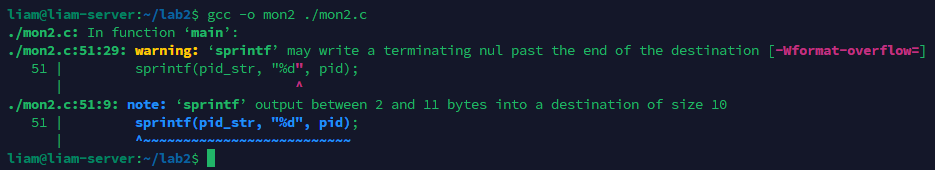
\includegraphics[width=0.8\textwidth]{mon2_compilation.png}
    \caption{Compilation of \texttt{mon2.c}}
    \label{fig:mon2_compile}
\end{figure}

\begin{figure}[H]
    \centering
    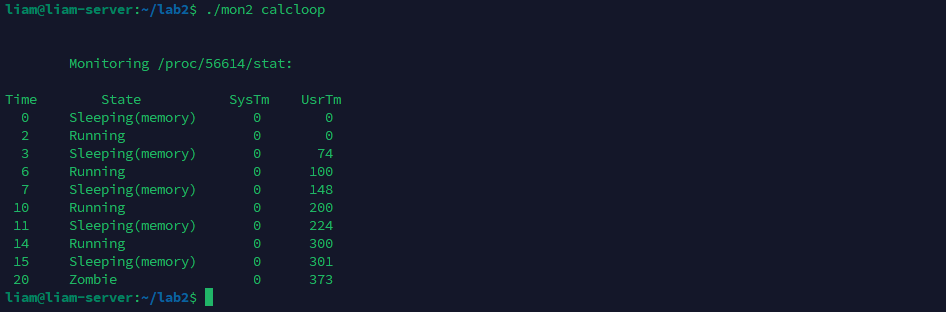
\includegraphics[width=0.8\textwidth]{mon2_output.png}
    \caption{Execution of \texttt{mon2 calcloop} showing filtered output}
    \label{fig:mon2_output}
\end{figure}

\begin{figure}[H]
    \centering
    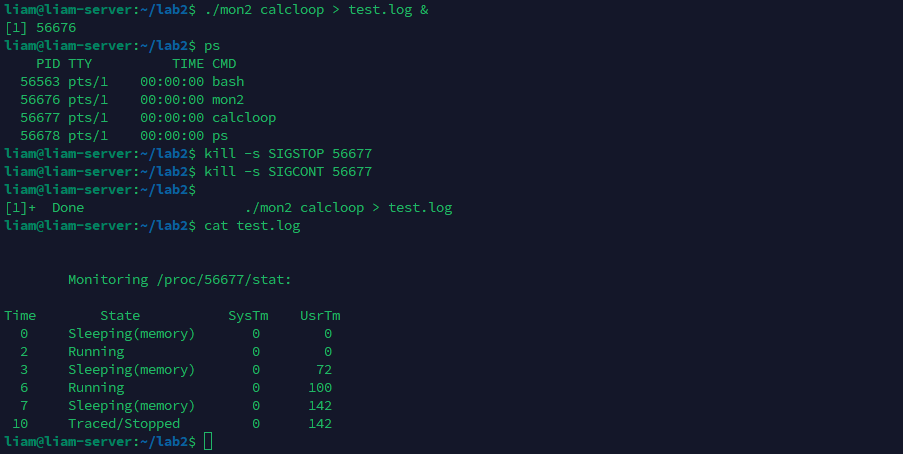
\includegraphics[width=0.8\textwidth]{mon2_signals.png}
    \caption{Sending signals to \texttt{calcloop} and observing output}
    \label{fig:mon2_signals}
\end{figure}

\begin{figure}[H]
    \centering
    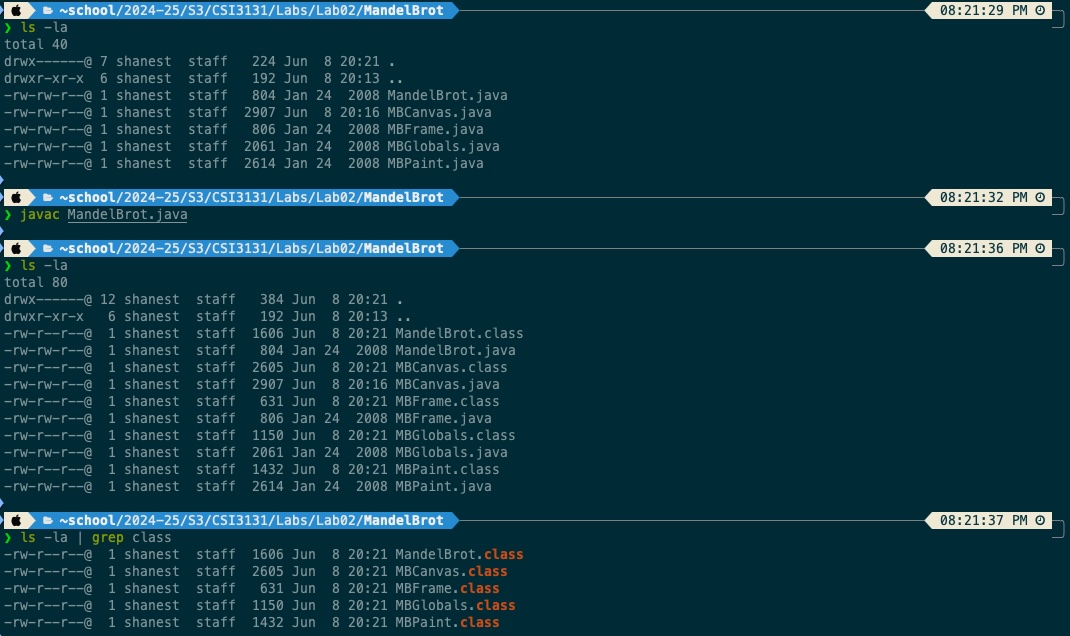
\includegraphics[width=0.9\textwidth]{lab02-img01}
    \caption{Successful compilation of Java Mandelbrot application}
    \label{fig:java_compile}
\end{figure}

\begin{figure}[H]
    \centering
    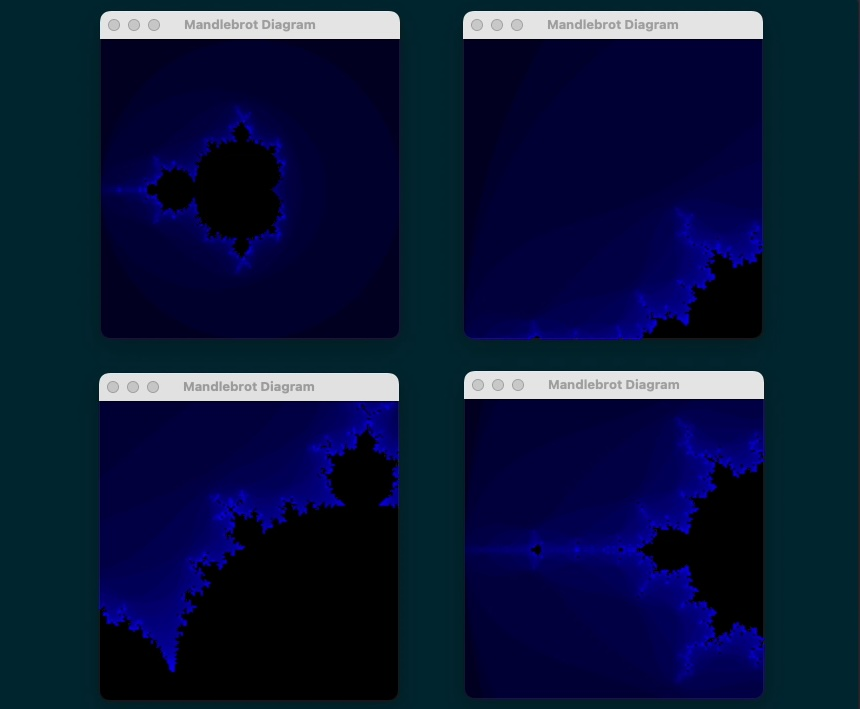
\includegraphics[width=0.75\textwidth]{lab02-img02}
    \caption{Four different Mandelbrot views using different parameters}
    \label{fig:mandelbrot_views}
\end{figure}

\begin{figure}[H]
    \centering
    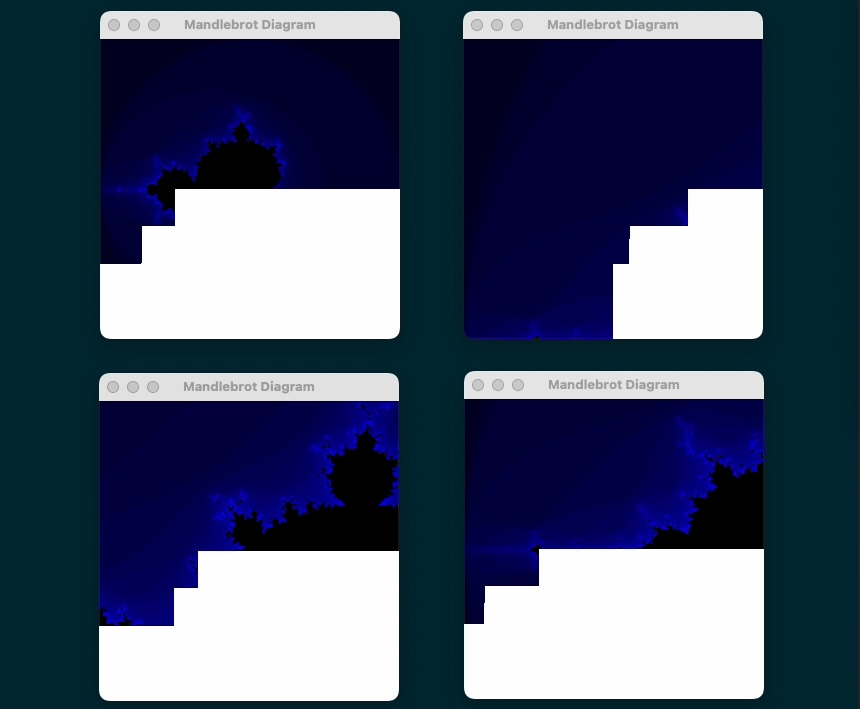
\includegraphics[width=0.75\textwidth]{lab02-img03}
    \caption{Initial rendering behavior without threading (sequential fill)}
    \label{fig:mandelbrot_seq}
\end{figure}

\begin{figure}[H]
    \centering
    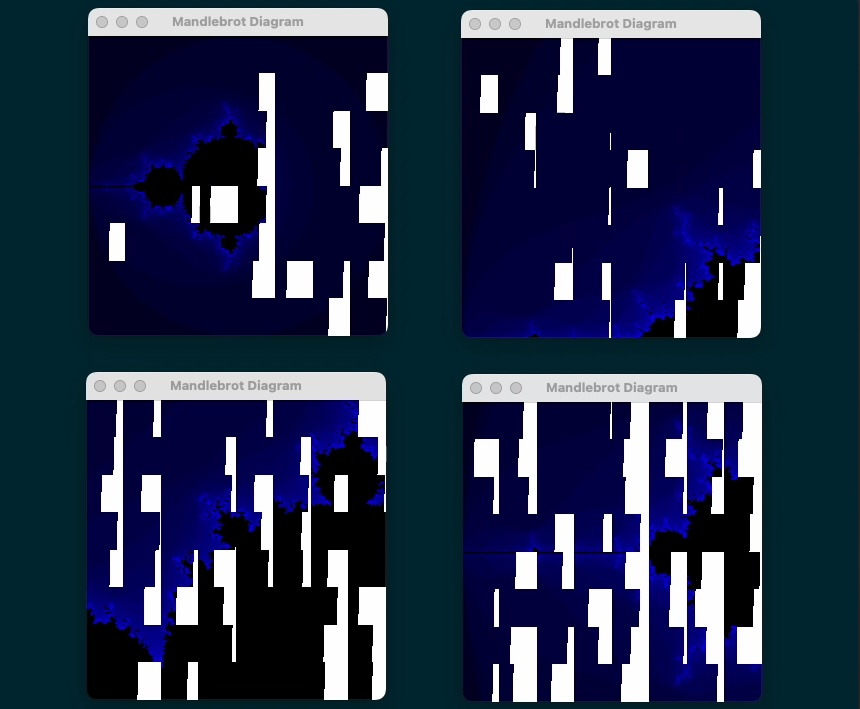
\includegraphics[width=0.85\textwidth]{lab02-img04}
    \caption{Rendering with Java Threads – faster and more parallel}
    \label{fig:mandelbrot_threads}
\end{figure}

\begin{figure}[H]
    \centering
    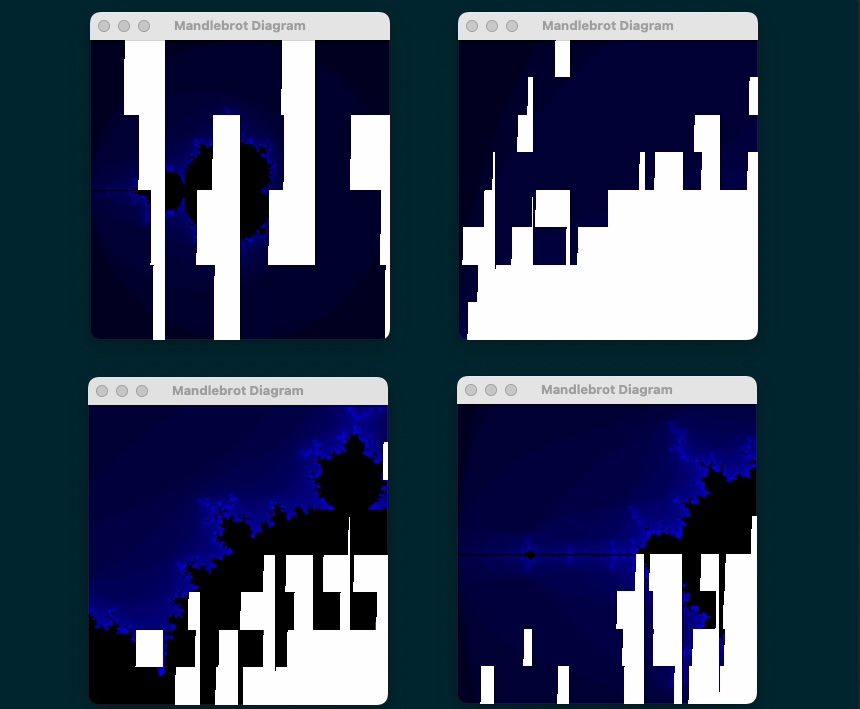
\includegraphics[width=0.85\textwidth]{lab02-img05}
    \caption{Rendering with Thread Pool – stable and efficient}
    \label{fig:mandelbrot_pool}
\end{figure}

\end{document}